\section{Validazione e auto-valutazione}
Successivamente in questo capitolo verranno descritti brevemente alcuni tra gli strumenti utilizzati per effettuare test sul codice sviluppato.\\[\baselineskip]\indent
Oltre a questi tools sono stati effettuati vari test con utenti durante le diverse fasi di implementazione. Basandosi sul bacino di utenti per il quale è stato pensato il sistema, sono state consultate per questi test persone interne all'università, anche iscritte ad altri corsi e quindi senza uno specifico background informatico.
Nelle prime fasi sono state richieste consulenze riguardo le scelte grafiche, presentando alcuni wireframes, e per quanto riguarda le specifiche a livello di regole di gioco e usabilità. Successivamente sono stati effettuati test di accessibilità chiedendo di accedere al sistema da dispositivi diversi e testare le funzionalità basilari come registrazione, autenticazione e persistenza delle sessioni. Nelle fasi finali i test sono stati impostati come vere e proprie demo di scenari di utilizzo reali, giocando partite complete toccando tutte le funzionalità implementate.



\subsection{Requisiti}
Qui di seguito verranno riportati gli elenchi presentati in fase di definizione dei requisiti analizzando quali di essi siano stati soddisfatti dal livello di implementazione raggiunto.
\paragraph{Requisiti funzionali}

\begin{itemize}[label={\checkmark}]
    \item accedere al sistema tramite credenziali univoche
    \item creare un nuovo party
    \item unirsi a un party esistente
    \item finalizzare il party e accedere alla lobby 
    \item avviare la partita
    \item selezionare un giocatore da uccidere/accusare
    \item visualizzare il risultato a partita terminata
\end{itemize}

I due requisiti funzionali identificati in fase di analisi come opzionali sono stati alla fine soddisfatti, in quanto il sistema permette sia di personalizzare le impostazioni della partita, sia di salvarla al termine della stessa.
\begin{itemize}[label={\checkmark}]
    \item (opzionale) selezionare la tipologia di partita
    \item (opzionale) salvare il risultato
\end{itemize}

\paragraph{Requisiti non funzionali}
\begin{itemize}[label={\checkmark}]
    \item il sistema dovrà essere scalabile
    \item l'architettura ibrida dovrà essere gestita in maniera efficiente
    \item la comunicazione dovrà essere “sicura” tra i peers e il server
    \item il sistema dovrà essere in grado di gestire in maniera corretta la connessione e disconnessione degli utenti durante il gioco
\end{itemize}

\subsection{Deliverables}
Al termine dello sviluppo gli artefatti prodotti sono stati:

\begin{itemize}[label={\checkmark}]
    \item Il database
    \item Il Server
    \item Il Client WEB
\end{itemize}
\begin{itemize}[label={$\times$}]
    \item Il Client Mobile
\end{itemize}

\subsection{Redux DevTools}
Per effettuare i test necessari a verificare che lo stato dell'applicazione fosse correttamente gestito sono stati usati gli strumenti offerti da Redux DevTools \cite{githubGitHubReduxjsreduxdevtools}.
Questi strumenti per sviluppatori permettono di migliorare il flusso di sviluppo di Redux o qualsiasi altra architettura che gestisca cambiamenti di stato. Può essere utilizzato come estensione per i principali browser, Chrome, Edge e Firefox, come app standalone oppure come componente React integrato nel client.

\begin{figure}[H]
\centering
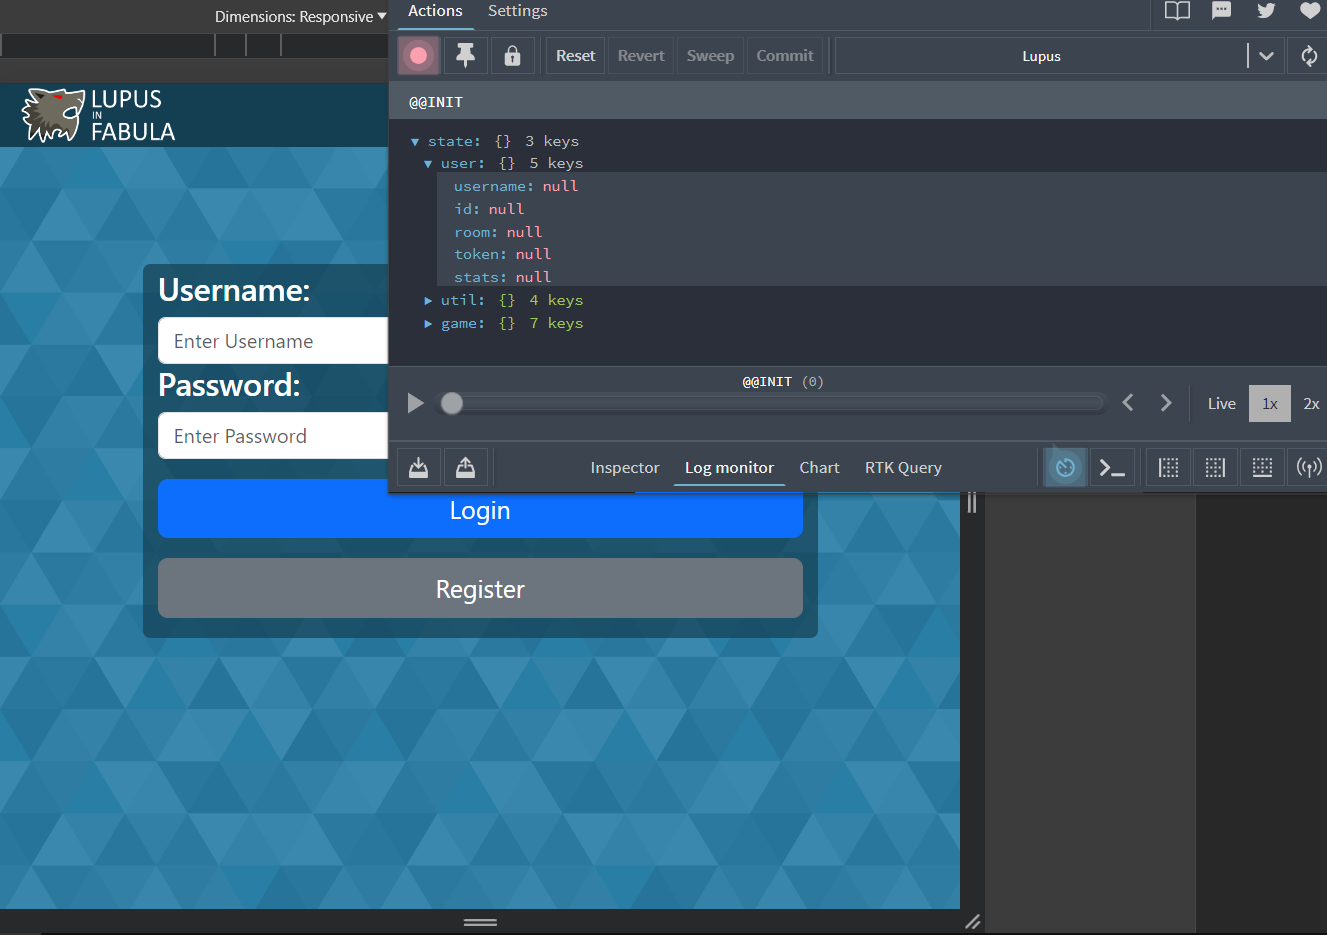
\includegraphics[width=0.9\textwidth]{img/screen/redux_devtools_usage.png}
\caption{Redux DevTools in uso}
\label{fig:reduxDevTools}
\end{figure}

Per lo sviluppo di questo progetto è stata utilizzata l'estensione messa a disposizione per Chrome, come mostrato nell figura \ref{fig:reduxDevTools}, nella quale è possibile vedere lo stato in tempo reale di Redux.

\begin{figure}[H]
\centering
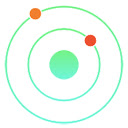
\includegraphics[width=0.3\textwidth]{img/logos/redux_devtool.jpg}
\caption{Redux DevTools logo}
\label{fig:reduxDevToolsLogo}
\end{figure}


\subsection{Axe DevTools}

Per testare aspetti di accessibilità sono stati invece utilizzati gli strumenti messi a disposizione da axe DevTools \cite{dequeDevToolsDeveloper}.
Questi tools permettono, sempre attraverso un'estensione disponibile per il browser Chrome, di analizzare vari aspetti di accessibilità relativi a una specifica pagina web o a una sua sottoparte. 

L'utilizzo dei tools è visibile nella figura \ref{fig:axeDevTools}, nella quale si può inoltre osservare la struttura di suddivisione utilizzata per attribuire un livello di gravità al problema riscontrato.


\begin{figure}[H]
\centering
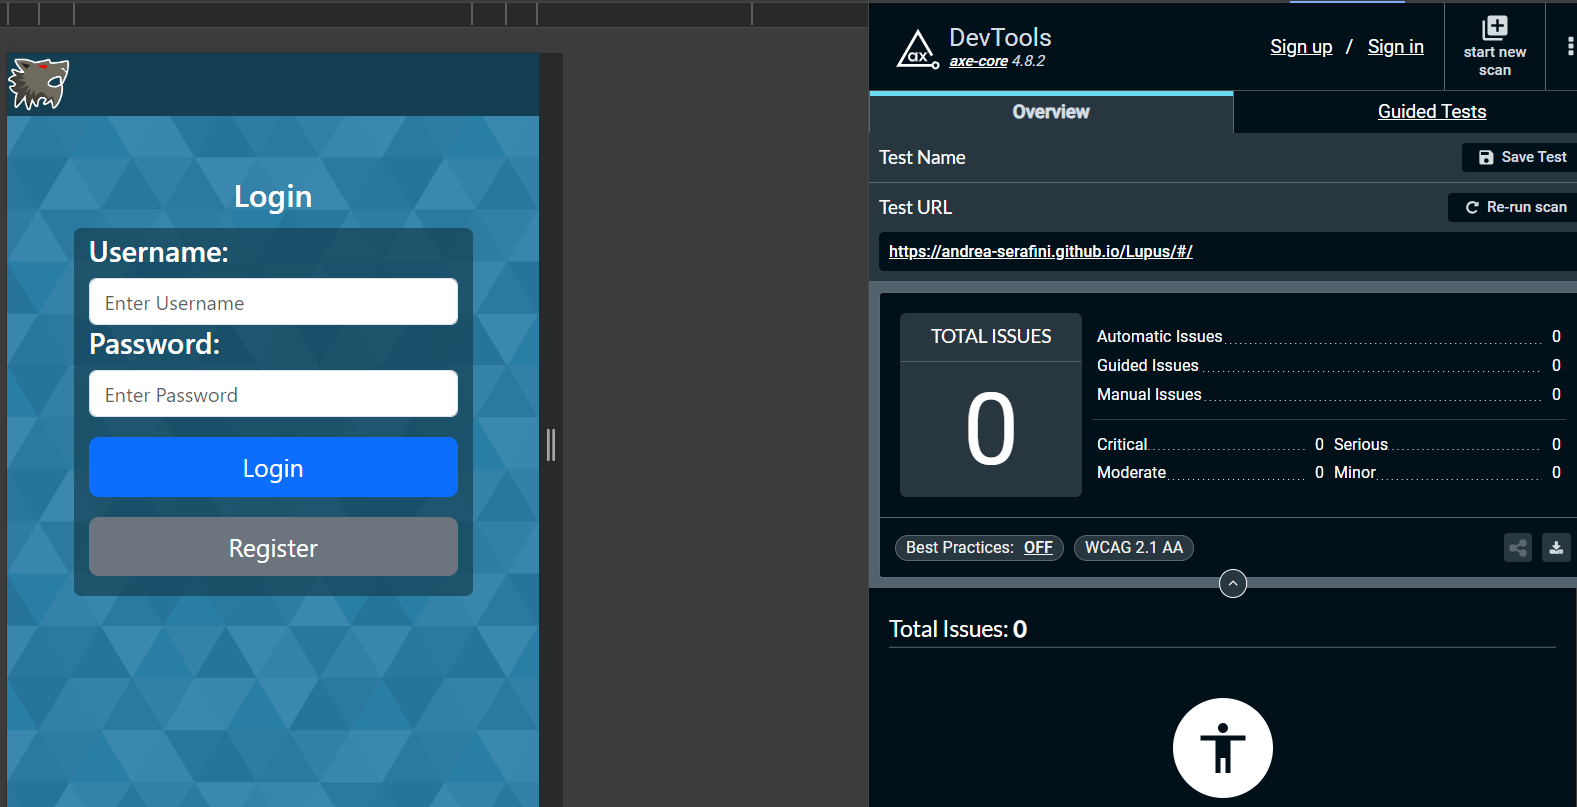
\includegraphics[width=\textwidth]{img/screen/axe_devtools_usage.png}
\caption{Axe DevTools in uso}
\label{fig:axeDevTools}
\end{figure}

Il set di tool di cui ci siamo serviti per monitorare ed eventualmente correggere questioni riguardanti l'accessibilità nel presente applicativo. Axe DevTools è un insieme di strumenti leader del settore, che permette tramite un'estensione installabile direttamente su browser di ispezionare una pagina web o sottoparti di essa allo scopo di individuare problemi di accessibilità. Il tool poi procede con il suddividere i problemi in varie categorie a seconda della gravità dei problemi eventualmente riscontrati:

\begin{figure}[H]
\centering

\includegraphics[width=0.4\textwidth]{img/logos/axeDevtools_logo.png}
\caption{Axe DevTools logo}
\label{fig:axeDevToolsLogo}
\end{figure}


\subsection{Lighthouse}
Lighthouse è uno strumento automatizzato completamente open-source pensato per migliorare le prestazioni, la qualità e la correttezza delle applicazioni Web \cite{githubLighthouse}.

Durante il controllo di una pagina, questo tool esegue una serie di test automatizzati e genera quindi un rapporto sul rendimento di quest'ultima, visibile nella figura \ref{fig:lighthouseReport}. Da qui è possibile utilizzare eventuali test falliti come indicatori di quali azioni si possano intraprendere per migliorare la propria applicazione.

\begin{figure}[H]
\centering
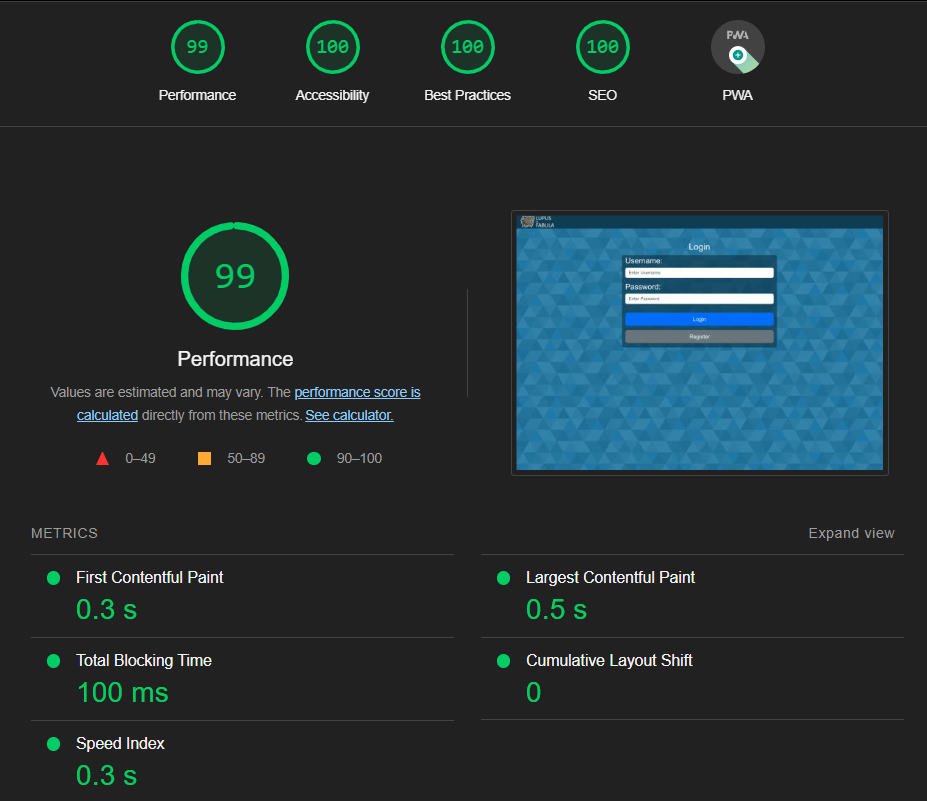
\includegraphics[width=0.8\textwidth]{img/screen/lighthouse_usage.png}
\caption{Lighthouse in uso}
\label{fig:lighthouseReport}
\end{figure}

\begin{figure}[H]
\centering

\includegraphics[width=0.3\textwidth]{img/logos/lighthouse_logo.png}
\caption{Lighthouse logo}
\label{fig:lighthouseLogo}
\end{figure}
